\section{Jacobian Matrix Compression}
\label{sec:jacobian-matrix-compression}


The main goal of Jacobian matrix compression is minimization of a number of non-linear function evaluations which are usually quite expensive computational operations. The minimization is performed by means of efficient treatment of non-zero entries of a sparse matrix. The problem is also known as matrix partitioning.\\


In the general case, a finite difference method can be used to compute a Jacobian matrix approximation in the following way:\\

\begin{equation} \label{eq:matrix-compression-1}
	\frac{1}{\epsilon} (F(y + \epsilon e_{k}) - F(y)) \approx J(y) e_{k}, \: \: \: 1 \leq k \leq N
\end{equation}

where $F : \mathbb{R}^{N} \rightarrow \mathbb{R}^{N}$  is a non-linear function; $e_{k} \in \mathbb{R}^{N}$ is the k\textit{th} coordinate unit vector, $\epsilon$ is a small step size.\\


Equation \ref{eq:matrix-compression-1} does not exploit Jacobian matrix sparsity and thus such estimation of the Jacobian matrix requires $N$ function evaluations.\\


\figpointer{\ref{fig:example-of-matrix-compression}}
\begin{figure}[htpb]
  \centering
  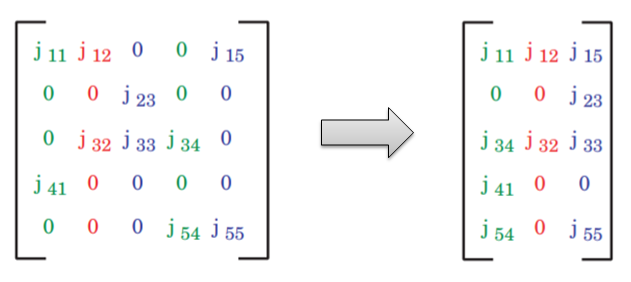
\includegraphics[width=0.55\textwidth]{figures/chapter-3/matrix-compression-example.png}
\caption[An example of matrix coloring and compression]{An example of matrix coloring and compression, \cite{gebremedhin2005color}}
\label{fig:example-of-matrix-compression}
\end{figure}


A compression algorithm is based on a notion of \textit{structurally orthogonal} columns i.e. columns which do not share any non-zero entry in a common row. Figure \ref{fig:example-of-matrix-compression} shows an example of matrix compression where each color denotes independent \textit{structurally orthogonal} columns.\\


% Curtis, Powell, and Reid [35] were the first to observe in 1974 that sparsity can be employed in this way to reduce the number of function evaluations needed to estimate the Jacobian.


Having obtained a compressed form of the Jacobian, another set of vectors $d \in \mathbb{R}^{N}$, also known as seed vectors, can be used to perform function perturbations instead of unit vectors $e_{k}$. A seed vector $d$ has 1’s in components corresponding to the indices of columns in a structurally orthogonal group of columns, and zeros in all other components \cite{gebremedhin2005color}. By differencing the function $F$ along the vector $d$, one can simultaneously determine the nonzero elements in all of these columns through one additional function evaluation at $F(y+d)$ \cite{gebremedhin2005color}.\\


It is obvious the algorithm requires to partition a matrix into the fewest amount of groups, colors, in order to achieve the most of efficiency. It means it is a NP-hard problem and, therefore, a huristical approach is required. \citeauthor{gebremedhin2005color}, in  \cite{gebremedhin2005color}, conducted one of the most recent studies in this field and summarized different matrix partitioning algorithms proposed over the last 20 years. Currently, a Jacobian matrix compression algorithm has been successfully implemented in \acrshort{nut} by means of the corresponding built-in \acrshort{petsc} subroutines. The algorithm is used by  \acrshort{athlet} via the corresponding \acrshort{nut} interface.\\ %through a \acrshort{nut} interface.\\


% unequal length of \acrshort{mpi} messages 
Figure \ref{fig:matrix-partitioning-example} shows an illustrative example of an efficient matrix partitioning where an initial 100 by 100 Jacobian matrix is transformed into its 100 by 28 compressed form using 28 distinct colors. It can be clearly observed from the figure that column vector lengths of the compressed Jacobian form are gradually decreasing. Figure \ref{fig:matrix-column-distribution} provides a detailed and clear view in the problem, using data from Figure \ref{fig:matrix-partitioning-example} as an example, where bars represent the corresponding column lengths.\\


\figpointer{\ref{fig:matrix-partitioning-example}}
\begin{figure}[htpb]
  \centering
  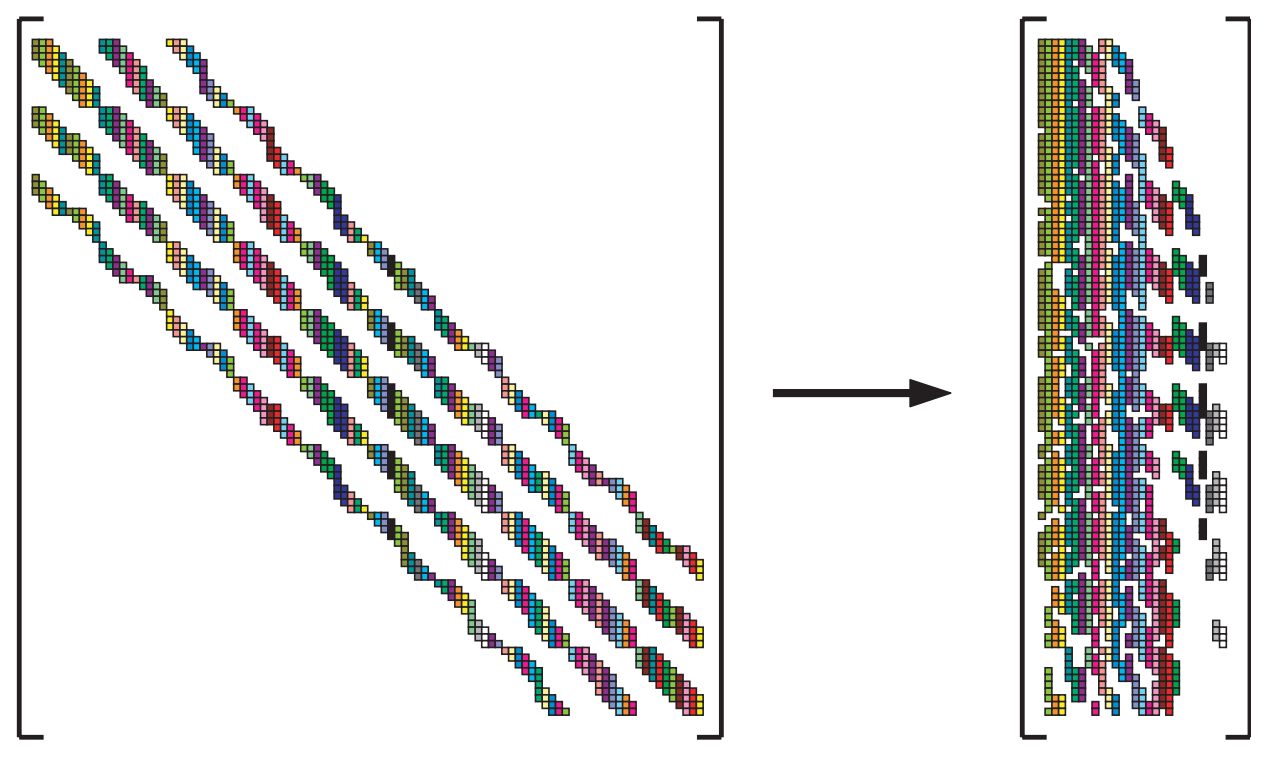
\includegraphics[width=0.8\textwidth]{figures/matrix-compression.png}
  \caption[An example of an efficient Jacobian matrix partitioning]{An example of an efficient Jacobian matrix partitioning, \cite{gebremedhin2005color}} \label{fig:matrix-partitioning-example}
\end{figure}


\begin{figure}[htpb]
  \centering
  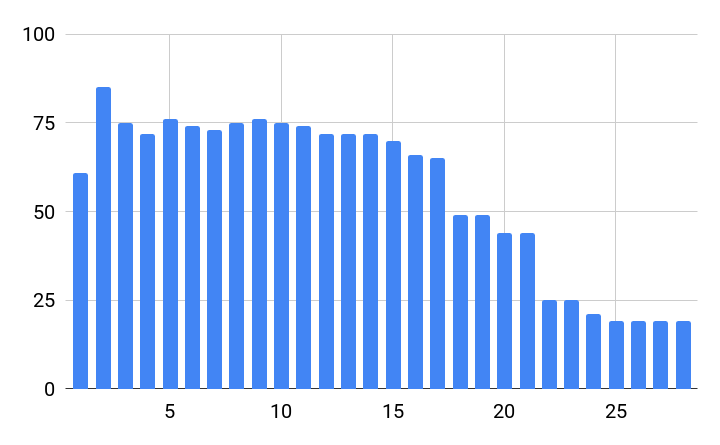
\includegraphics[width=0.7\textwidth]{figures/matrix-compression-2.png}
  \caption{A column-length distribution of the example depicted in Figure \ref{fig:matrix-partitioning-example}} \label{fig:matrix-column-distribution}
\end{figure}


According to the \acrshort{athlet}-\acrshort{nut} coupling design, each column is transfered to \acrshort{nut} by means of the synchronous 3-way handshake procedure, described in Section \ref{sec:athlet-nut-coupling}, immediately after its evaluation. Thus,  Figure \ref{fig:matrix-column-distribution} determines the communication pattern during the Jacobian matrix transfer for the example shown in Figure \ref{fig:matrix-partitioning-example}.\\


% listing
Code Listings \ref{lst:athlet-grs-defaul:athlet} and \ref{lst:athlet-grs-defaul:nut} represent the default implementation of a compressed Jacobian matrix transfer between \acrshort{athlet} and \acrshort{nut}. This code is used as a baseline for the remaining part of the study.\\


All \textbf{code listings}, presented in this part of the study, are written in \textbf{pseudocode} and intended for convenience of reading. The aim is to show and display the main ideas skipping non-relevant parts of the actual source code. The \textbf{pseudocode} is a mixture of several programming languages, namely: \textbf{Python}, \textbf{C/C++}, \textbf{Fortran}, (\textbf{\acrshort{mpi}}).\\


\begin{minipage}{\linewidth}
\begin{lstlisting}[language=python, caption={Pseudocode of the original \acrshort{athlet}-\acrshort{nut} coupling: \acrshort{athlet} part}, frame=single, label={lst:athlet-grs-defaul:athlet}]
# GIVEN PARAMETERS:
# acomm - the athlet communicator
# acomm_id - athlet identification number 
# y - known vector
# N - problem size
# COO - compressed matrix coordinate format

eps = 1e-4
center = f(y)
column = zeros(N)

# compute Jacobian and send it to NUT column-by-column
for seed_vector in seed_vectors:

	# compute the next column
	vector = evaluate_jacobian(f, seed_vector, center, eps)
	
	length = perturbed_vector.length
	signal = [encode("add_to_jacobian"), acomm_id]
	
	# perform 3-way handshake
	MPI_Send(signal, 2, int, acomm.head, acomm)
	
	# broadcast jacobian column length
	MPI_Bcast(length, 1, int, acomm.head, acomm)
	
	# broadcast jacobian column
	MPI_Bcast(vector.data, length, COO, acomm.all, acomm)
	

\end{lstlisting}
\end{minipage}



\begin{minipage}{\linewidth}
\begin{lstlisting}[language=python, caption={Pseudocode of the original \acrshort{athlet}-\acrshort{nut} coupling: \acrshort{nut} part}, frame=single, label={lst:athlet-grs-defaul:nut}]
# N - problem size
# J - allocated distributed jacobian matrix
# COO - compressed matrix coordinate format
nut_running = True

while nut_running:
	if rank in heads:
		
		# receive request
		MPI_Recv(signal, 2, int, NUT_WORLD.any_client, NUT_WORLD)
		
		comm = my_comm_list[signal[1]]
		if (comm not None):
			# posses resources
			MPI_Bcast(signal, 2, int, comm.all, comm)
		else:
			continue
		
	else:
		MPI_Recv(signal, 2, int, NUT_WORLD.any_head, NUT_WORLD)
		
	# decode request
	comm = my_comm_list[signal[1]]
	if (comm not None):	
		request = decode(signal[0])
	
		case(request):
			...
			if (request == "exit"):
				# beak while loop			
				nut_running = False
			
			if (request == "add_to_jacobian"):
				# receive jacobian column length
				MPI_Recv(length, 1, int, comm.client, comm)
	
				# receive row jacobian column
				MPI_Recv(elements, length, COO, comm.client, comm)

			
				for i in range(0, length):
					if (local_min < elements[i].row < local_max):
						J.insert(elements[i])
		...

\end{lstlisting}
\end{minipage}




%The effect of color size reduction is the particularly field of interest in this study because it determines the communication pattern between the client and server. It is well known that sending small messages can lead to performance deterioration due to not full resource utilization. In this case we consider the network bandwidth as the main resource.\\

%\emph{example of jacobian evaluation}


 

% and there exist several algorithms which can tackle it, namely: [reference to the book]

%The coloring technique 
